\chapter*{Template} % l'asterisco fa in modo che non compaia "Capitolo 1"
\addcontentsline{toc}{chapter}{Template} % aggiunge il capitolo al TOC
\minitoc % Indice del capitolo
% \mtcskip
% \minilof % Lista delle figure
% \mtcskip
% \minilot % Lista delle tabelle


\lettrine{Q}{uesto} e' un template latex per scrivere il documento finale di tesi. In questo capitolo spieghero' brevemente quali sono i pacchetti al momento inclusi in questo template~\marginpar{Questa e' una nota a margine}, insieme ad alcuni dei comandi base utili alla scrittura del documento.


Per i comandi piu' basilari, come: la selezione della classe del documento, stampare l'indice, o aggiungere altri capitoli; fare riferimento al file \verb|main.tex|.

\section{Sezione 1}

\section{Sezione 2}

\subsection{Figure}

\mbox{} serve a non spezzare il contenuto, andando a capo

Questo e' il modo per inserire una sola figura con la caption~\cite{doc:unityengine}

% h = here, t = top, b = bottom, p = page of float
\begin{figure}[!ht]
    \centering
    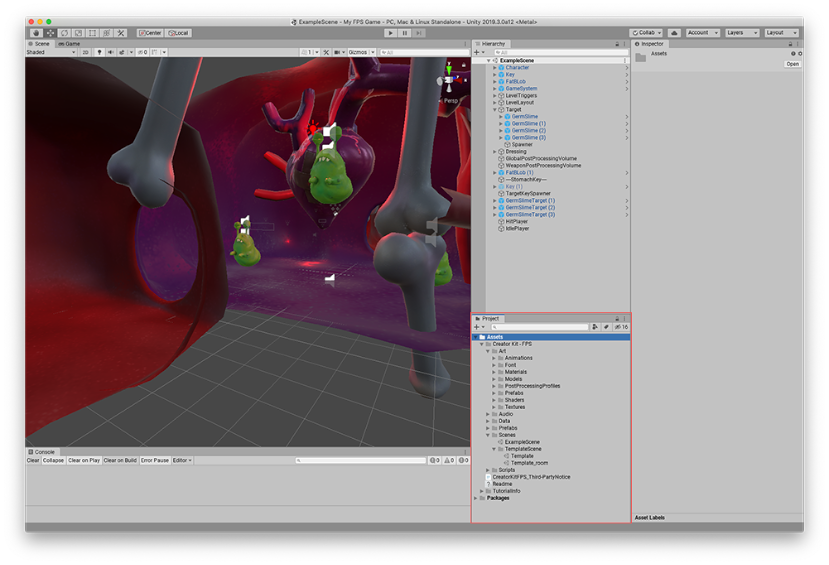
\includegraphics[width=0.95\columnwidth]{gfx/imgs/introduction/unity_editor.png}
    \caption{Unity Engine Editor.}
    \label{fig:unity-engine-editor}
\end{figure}

Mentre questo se vogliamo inserire due figure ognuna con la propria caption:

\begin{figure}[!b]
    \begin{subfigure}{.49\textwidth}
      \centering
      % include first image
      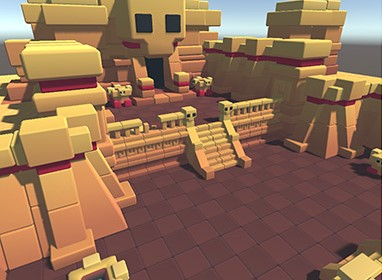
\includegraphics[width=.95\linewidth]{gfx/imgs/introduction/perspective_camera.jpg}
      \caption{Vista in proiezione prospettica.}
      \label{fig:perspective-camera}
    \end{subfigure}
    \begin{subfigure}{.49\textwidth}
      \centering
      % include second image
      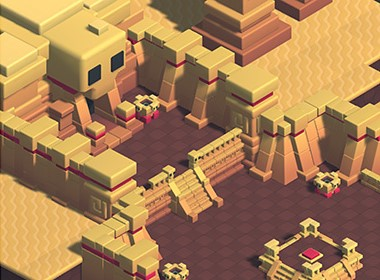
\includegraphics[width=.95\linewidth]{gfx/imgs/introduction/ortho_camera.jpg}
      \caption{Vista in proiezione ortografica.}
      \label{fig:ortho-camera}
    \end{subfigure}
    \caption{Tipi di camera projection.}
    \label{fig:camera-projection}
\end{figure}]


\lstinputlisting{chapters/template.tex} % per importare un file